\subsection{Transfer from synthetic benchmarks to cytometry}
\label{sec:results-cytometry}

\textbf{RQ4 asks whether StrataSCAN generalizes from controlled synthetic datasets to real cytometry data.}
We evaluated all nine methods on 13 cytometry datasets (Levine, Mosmann, Nilsson, and ten Samusik samples) under the frozen \texttt{target-discovery-v1} contract. Reference populations were matched to predicted clusters one-to-one by Hungarian optimization of pairwise F1. Macro target F1 was the primary endpoint; target purity, coverage, and discovery at purity $\geq0.90$ and coverage $\geq0.10$ were supporting endpoints. Because unlabeled cytometry events are not verified noise, background abstention was retained only as a diagnostic and excluded from the primary comparison. The resulting matrix contained 117 attempted cells (13 datasets $\times$ 9 methods), of which 99 completed successfully.

\begin{figure}[t]
  \centering
  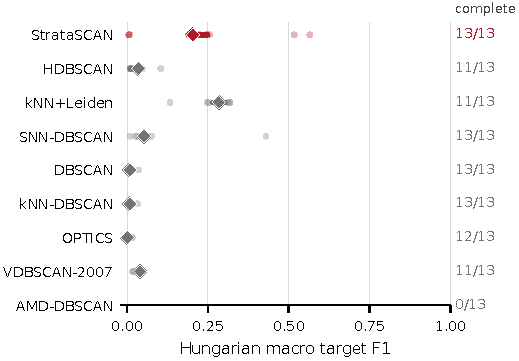
\includegraphics[width=\columnwidth]{outputs/rq4_cytometry/fig_rq4_cytometry.pdf}
  \caption{Biological target recovery across 13 cytometry datasets under the frozen \texttt{target-discovery-v1} contract. Small points denote successful dataset-level macro target F1 values, diamonds denote medians, and thick segments denote interquartile ranges; right-hand labels report successful executions out of 13. F1 uses Hungarian one-to-one matching with pairwise F1 as the assignment objective. Failed executions are absent (NA), not encoded as zero; background-abstention diagnostics are excluded.}
  \label{fig:rq4-cytometry}
\end{figure}

StrataSCAN completed all 13 datasets and obtained a median macro target F1 of 0.202 (IQR 0.008--0.244), the highest median among methods that completed every dataset (Fig.~\ref{fig:rq4-cytometry}). Its median target purity and coverage were 0.437 and 0.244, respectively. StrataSCAN achieved the highest F1 on Levine (0.190 versus 0.036 for the best successful baseline) and Nilsson (0.517 versus 0.133). kNN+Leiden produced the highest successful-run median F1, 0.284 (IQR 0.265--0.302), and led on all ten Samusik samples, but timed out on Levine and Mosmann and therefore completed 11/13 datasets. Its higher coverage (median 0.476) was accompanied by lower purity (median 0.225) than StrataSCAN. HDBSCAN also completed 11/13, VDBSCAN-2007 completed 12/13, and AMD-DBSCAN completed none; failed cells were treated as missing, never as zero-quality results.

The stricter discovery endpoint exposed a complementary trade-off. StrataSCAN produced at least one qualifying high-purity discovery in seven of the ten Samusik samples, whereas kNN+Leiden produced none under the same threshold. SNN-DBSCAN produced qualifying discoveries in six Samusik samples and was strongest on Mosmann, giving it the largest mean discovery rate (0.096 versus 0.035 for StrataSCAN). Thus, the cytometry evidence supports reliable but dataset-dependent transfer: StrataSCAN combines complete execution with the strongest median target recovery among full-completion methods and a more purity-oriented solution than kNN+Leiden, but it is not uniformly best across biological datasets.

\textit{Answer to RQ4:} StrataSCAN transfers to real cytometry data with complete execution and the highest median target F1 among methods completing all 13 datasets, while its losses on Mosmann and the Samusik series show that this advantage is reliability- and purity-oriented rather than universal.

